% \makeatletter % Use \makeatletter to make '@' a letter
% \def\input@path{{../}} % Define input path to parent directory
% \makeatother % Restore default category code of '@'

\documentclass[../Tesi_Jiahao_Miao_986136.tex]{subfiles}
\begin{document}

\chapter{Resummed Calculations for Thrust}\label{ch:calculations}

We now turn to one of the many results of the present work: the calculation of the resummation coefficients $f_i(\lambda)$ of the
Sudakov form factor $\exp{\mathcal{F}}$. To compute the $f_i(\lambda)$ functions, equation \cref{eq:master formula} is used, which
requires knowledge of the $\mu$-dependence of the QCD running coupling $\alpha_s(\mu)$.
We therefore proceed firstly to calculate the running coupling $\alpha_s(\mu)$ from LO up to N$^4$LO because the QCD $\beta$-function is known up to five loops \cite{Herzog_2017}. 
We then use the obtained results to calculate the $f_i(\lambda)$ functions up to $i = 5$.

\section{QCD running coupling} \label{sec:QCD_running_coupling}

A surpring effect of the renormalization procedure is that, after renormalization, the coupling "constants" are not constant
at all, but depend on the energy.

One way to understand this is the following: Classically, the Coulomb potential between two sources is then given by $V = \frac{\alpha}{r}$, 
characterized by a universal coefficient -- the coupling constant $\alpha$, which 
quantifies the force between two static bodies of unit “charge” at distance $r$,
\textit{i.e.}, the electric charge for QED, the color charge for QCD, the weak isospin
for the weak force, or the mass for gravity. Consequently, the coupling $\alpha$ is defined
as being proportional to the elementary charge squared, \textit{e.g.}, $\alpha_{em} \equiv \frac{e^2}{4\pi}$ where 
$e$ is the elementary electric charge, or $\alpha_s \equiv \frac{g^2}{4\pi}$ where $g$ is the elementary gauge field
coupling in QCD.
In the non-relativistic limit of QCD, $\frac{1}{r}$ is the coordinate-space representation
for the propagator of the gluon (force carrier) at leading-order in perturbation
theory: in momentum space, the analogous propagator is proportional to $\frac{1}{q^2}$, where q is
the boson 4-momentum ($Q^2=-q^2>0$).

For sources interacting weakly, the one-boson exchange representation of interactions
is a good approximation. However, when interactions become strong, higher orders in perturbation theory become noticeable and the
$\frac{1}{r}$ law no longer stands. In such cases, it makes good physics sense to fold the extra r-dependence
into the coupling, which thereby becomes $r$, or equivalently $Q^2$, dependent.

Another way to view this is that the running of the coupling is due to vacuum polarization. The vacuum is not empty, but is filled 
with virtual particles that are constantly created and annihilated which can interact with the propagating particles,
leading to a modification of the interaction strength. 

While in QED, the extra $r$-dependence comes only from the vacuum polarization. In QCD, 
$\alpha_s$ receives contributions from the vacuum polarization and from gluon self-interactions since the gluon 
has a color charge.

The two couplings have opposite trends: the QED coupling increases with energy and the theory could eventually become strongly
coupled at extremely high energies, whereas the opposite happens for the QCD coupling as it is large at low
energies and decreases with energy. This property of being weakly coupled at high energies is
known as \emph{asymptotic freedom} and it means that perturbative calculations in QCD can be used at high energies where $\alpha_s$ becomes small enough that a power expansion is meaningful.

In the framework of perturbative QCD (\emph{pQCD}), predictions for observables are expressed in
terms of the renormalized coupling $\alpha = \alpha (\mu^2)$, a function of an unphysical renormalization scale
$\mu_R$. 
The coupling satisfies the following renormalization group equation (RGE):

\begin{equation}\label{eq:RGE}
    \mu^2 \frac{d\alpha}{d\mu^2} = \beta(\alpha) = -\left( b_0 \alpha^2 + b_1 \alpha^3 + b_2 \alpha^4 + \ldots \right),
\end{equation}

where $b_0$ is the 1-loop $\beta$-function coefficient,  
$b_1$ is the 2-loop coefficient, 
$b_2$ is the 3-loop coefficient.
$C_A = 3$ and $C_F = \frac{4}{3}$ are the Casimir operators of the adjoint and fundamental representations of $SU(3)$,
$T_R = \frac{1}{2}$ is the trace normalization, $n_f$ is the number of active quark flavors. 

It is not possible to solve \cref{eq:RGE} as it is for two reasons: only the first few $b_n$ 
coefficients are known (up to $b_4$); the exact equation becomes more and more complicated 
as more terms of the series are included, making it impossible to obtain an analytic solution.

In order to solve both problems, the equation is solved in the following way: at first only $b_0$
is included and the obtained solution is called $\alpha_{\text{LO}}$ , as it will only contain a term proportional to
$\alpha$ ; then also $b_1$ is included and only terms up to the second order in $\alpha$ are kept to obtain $\alpha_{\text{NLO}}$ ;
this same procedure is used to obtain $\alpha_{\text{NNLO}}$ , $\alpha_{\text{N}^3\text{LO}}$ , $\alpha_{\text{N}^4\text{LO}}$ . There will be a complication in
calculating $\alpha_{\text{NLO}}$ and higher orders which will be explained and resolved in the following sections.

\subsection{One-loop running coupling and higher order corrections}

The one-loop running coupling $\alpha_{\text{LO}}$ is obtained by solving the RGE \cref{eq:RGE} with only the first term of the $\beta$-function:

\begin{equation}
    \mu^2 \frac{d\alpha}{d\mu^2} = - b_0 \alpha^2.
\end{equation}

This equation can be solved by separation of variables and imposing 
the boundary condition $\alpha(Q^2) = \alpha_s$:

\begin{equation}
   \int_{\alpha(Q^2)}^{\alpha(\mu^2)} \frac{\dd\alpha}{\alpha^2} = \int _{Q^2}^{\mu^2}-b_0 \frac{\dd\mu^2}{\mu^2},
\end{equation}

and one obtains:

\begin{equation}
    \alpha_{\text{LO}}(\mu^2) = \frac{\alpha_s}{1+b_0 \alpha_s \log(\frac{\mu^2}{Q^2})},
\end{equation}

in which one can observe the decreasing with energy trend of the running coupling (asymptotic freedom).  

It is useful to define the variable $\lambda_\mu = b_0 \alpha_s \log(\frac{\mu^2}{Q^2})$ so that:

\begin{equation}\label{eq:LO running coupling}
    \alpha_{\text{LO}}(\mu^2) = \frac{\alpha_s}{1+\lambda_\mu}.
\end{equation}

In order to obtain the two-loop running coupling $\alpha_{\text{NLO}}$, 
we need to solve the RGE with the first two terms of the $\beta$-function \cref{eq:RGE}:

\begin{equation}
    \mu^2 \frac{d\alpha}{d\mu^2} = - b_0 \alpha^2 - b_1 \alpha^3,
\end{equation}

but this equation is not solvable in a straightforward way as the one-loop equation, 
we have to use the perturbative approach. We can rewrite the equation as:

\begin{equation}
    \frac{d\alpha}{d\mu^2} = - \frac{b_0 \alpha^2}{\mu^2} ( 1 - \frac{b_1}{b_0} \alpha ),
\end{equation}

and expand the $\alpha$ term in the parenthesis as:

\begin{equation}
    \alpha = \alpha_{\text{LO}} + \delta \alpha,
\end{equation}

where $\alpha_{\text{LO}}$ is the one-loop running coupling and $\delta\alpha$ contains the higher order correction, one obtains:

\begin{equation}
    \frac{d\alpha}{d\mu^2} = - \frac{b_0 \alpha^2}{\mu^2} ( 1 - \frac{b_1}{b_0} \alpha_{LO} - \frac{b_1}{b_0} \delta\alpha).
\end{equation}

Observe that in parenthesis, by keeping 1 gave us the one-loop running coupling, by keeping $\frac{b_1}{b_0} \alpha_{LO}$ we can obtain the first order corrections
and $\delta\alpha$ are needed for higher order corrections. The equation to solve is then:

\begin{equation}
    \int_{\alpha_s}^{\alpha(\mu^2)} -\frac{\dd\alpha}{\alpha^2} = 
    \int _{Q^2}^{\mu^2} - b_0 \frac{ \dd\mu^2}{\mu^2} ( 1 - \frac{b_1}{b_0} \alpha_{LO}(\mu^2) ).
\end{equation}

Using \emph{Mathematica} \cite{Mathematica} to solve this equation, we obtain the two-loop running coupling:

\begin{equation}
    \alpha_{\text{NLO}}(\mu^2) = \frac{\alpha_s}{1+\lambda_\mu + \alpha_s \frac{b_1}{b_0} \log(1+\lambda_\mu)},
\end{equation}

in which the expansion in powers of $\alpha_s$ is not explicit. One can expand 
in powers of $\alpha_s$ by keeping $\lambda_\mu$ fixed and only keeping terms up to 
$\order{\alpha_s^2}$ by doing so one obtains:

\begin{equation}\label{eq:NLO}
    \alpha_{\text{NLO}}\qty(\mu^2) = \alpha_{\text{LO}}\qty(\mu^2) -\frac{b_1}{b_0} \alpha_{LO}^2\qty(\mu^2) \log(1+\lambda_\mu) + \mathcal{O}(\alpha_s^2) .
\end{equation}

We found the correction: 
\begin{equation}\label{eq:DNLO}
\delta\alpha_{\text{NLO}}\qty(\mu^2) = -\frac{b_1}{b_0} \alpha_{\text{LO}}^2\qty(\mu^2) \log(1+\lambda_\mu) .
\end{equation}

By repeating the same procedure, one can obtain the three-loop running coupling $\alpha_{NNLO}$ and so on.

In order to calculate higher order corrections, one need to be careful of the powers of $\alpha$ needed for the desired order, 
and the contributions to various orders of $\alpha_s$ may not be immediately apparent, but they are straightforward to compute.
Expand the running coupling in powers of $\alpha_s$ as: 
\begin{equation}
    \alpha = \alpha_{\text{LO}} + \delta\alpha_{\text{NLO}} + \delta\alpha_{\text{NNLO}} + \delta\alpha_{\text{N}^3\text{LO}} + \delta\alpha_{\text{N}^4\text{LO}} + \ldots,
\end{equation} 
with $\delta\alpha_{\text{NLO}} = \mathcal{O}(\alpha_s)$, $\delta\alpha_{\text{NLO}} = \order{\alpha_s^2}$, $\delta\alpha_{\text{NNLO}} = \mathcal{O}(\alpha_s^3)$,
$\delta\alpha_{\text{N}^3\text{LO}} = \mathcal{O}(\alpha_s^4)$, $\delta\alpha_{\text{N}^4\text{LO}} = \mathcal{O}(\alpha_s^5)$, and so on.

We present these contributions in the following table:
\begin{table}[htbp] %h= here, t=top, b=bottom, p=page
    \centering
    \caption{Contributions to different powers of $\alpha_s$.}
    % \scriptsize
    \begin{tabular}{c c c c c c c}
        \textbf{Power} & $\mathcal{O}(\alpha_s)$ & $\mathcal{O}(\alpha_s^2)$ & $\mathcal{O}(\alpha_s^3)$ 
        & $\mathcal{O}(\alpha_s^4)$ & $\mathcal{O}(\alpha_s^5)$\\
     
        $\alpha$ & $\alpha_{\text{LO}}$ & $\delta\alpha_{\text{NLO}}$ & $\delta\alpha_{\text{NNLO}}$ & $\delta\alpha_{\text{N}^3\text{LO}}$ & $\delta\alpha_{\text{N}^4\text{LO}}$  \\
        $\alpha^2$ &  & $\alpha_{\text{LO}}^2$ & $2\alpha_{\text{LO}}\delta\alpha_{\text{NLO}}$ & $\delta\alpha_{\text{NLO}}^2+2\alpha_{\text{LO}}\delta\alpha_{\text{NNLO}}$ &
        $2\alpha_{\text{LO}}\delta\alpha_{\text{N}^3\text{LO}}+3\alpha_{\text{LO}}\delta\alpha_{\text{NLO}}^2$ \\
        $\alpha^3$ &  & & $\alpha_{\text{LO}}^3$ & $3\alpha_{\text{LO}}^2 \delta\alpha_{\text{NLO}}$& $3\alpha_{\text{LO}}^2\delta\alpha_{\text{NNLO}}+3\alpha_{\text{LO}}\delta\alpha_{\text{NLO}}^2$  \\
        $\alpha^4$ &  & & & $\alpha_{\text{LO}}^4$ & $4 \alpha_{\text{LO}}^3 \delta\alpha_{\text{NLO}}$  \\
        $\alpha^5$ &  & & & & $\alpha_{\text{LO}}^5$ \\
    \end{tabular}
    \label{tab:contributions to different powers of alpha_s}
\end{table}

For the three-loop running coupling, the equation to solve is:

\begin{equation}
    \mu^2 \frac{d\alpha}{d\mu^2} = - b_0 \alpha^2(1 - \frac{b_1}{b_0} \alpha - \frac{b_2}{b_0} \alpha^2).
\end{equation}

One can substitute the expansion of $\alpha= \alpha_{\text{LO}}+\delta\alpha_{\text{NLO}}+\order{\alpha_s^2}$ in powers of $\alpha_s$ 
and retain only terms up to $\order{\alpha_s^2}$, with this prescription the equation to solve is:

\begin{equation}
    \int_{\alpha_s}^{\alpha(\mu^2)} -\frac{\dd\alpha}{\alpha^2} = 
    \int _{Q^2}^{\mu^2} - b_0 \frac{ \dd\mu^2}{\mu^2} ( 1 - \frac{b_1}{b_0} \alpha_{\text{NLO}}(\mu^2) - \frac{b_2}{b_0} \alpha_{LO}^2(\mu^2) ),
\end{equation}

solving the above integral yields the three-loop running coupling $\alpha_{NNLO}$:

\begin{equation}\label{eq:NNLO}
    \alpha_{\text{NNLO}}(\mu^2) = \alpha_{\text{LO}}\qty(\mu^2) + \delta\alpha_{\text{NLO}}\qty(\mu^2)+\delta\alpha_{\text{NNLO}}\qty(\mu^2),
\end{equation}

with 
\begin{equation}\label{eq:DNNLO}
    \delta\alpha_{\text{NNLO}}\qty(\mu^2) = \frac{\alpha_{\text{LO}}^3\qty(\mu^2)}{b_0^2}\left(b _1^2 \lambda_\mu -b_0 b_2 \lambda_\mu +b_1^2 \log ^2(1+\lambda_\mu )-b_1^2 \log (1+\lambda_\mu )\right).
\end{equation}

Similarly, one can obtain the four-loop running coupling $\alpha_{N^3LO}$ and five-loop running coupling $\alpha_{N^4LO}$

\begin{equation}\label{eq:N3LO}
    \alpha_{\text{N}^3\text{LO}}(\mu^2) = \alpha_{\text{LO}}\qty(\mu^2) + \delta\alpha_{\text{NLO}}\qty(\mu^2)+\delta\alpha_{\text{NNLO}}\qty(\mu^2)+\delta\alpha_{\text{N}^3\text{LO}}\qty(\mu^2),
\end{equation}

\begin{equation}\label{eq:DN3LO}
    \begin{split}
        \delta\alpha_{\text{N}^3\text{LO}}\qty(\mu^2) &= \frac{\alpha_{\text{LO}}^4\qty(\mu^2)}{2 b_0^3} \Bigl(-\left(b_1^3-2 b_0 b_2 b_1+b_0^2 b_3\right) \lambda _{\mu }^2\\
        &-\left(2 b_0^2 b_3-2 b_0 b_1 b_2\right) \lambda _{\mu }-2 b_1^3 \log ^3\left(\lambda _{\mu }+1\right)+5 b_1^3 \log ^2\left(1+\lambda _{\mu }\right)\\
        &+\left(2 b_0 b_1 b_2 \left(2 \lambda _{\mu }-1\right)-4 b_1^3 \lambda _{\mu }\right) \log \left(1+\lambda _{\mu }\right)\Bigr),
    \end{split}
\end{equation}

\begin{equation}\label{eq:N4LO}
    \alpha_{\text{N}^4\text{LO}}(\mu^2) = \alpha_{\text{LO}}\qty(\mu^2) + \delta\alpha_{\text{NLO}}\qty(\mu^2)+\delta\alpha_{\text{NNLO}}\qty(\mu^2)+\delta\alpha_{\text{N}^3\text{LO}}\qty(\mu^2) + \delta\alpha_{\text{N}^4\text{LO}}\qty(\mu^2),
\end{equation}

\begin{equation}\label{eq:DN4LO}
    \begin{split}
        \delta\alpha_{\text{N}^4\text{LO}} &= \frac{\alpha_{\text{LO}}^5}{6 b_0^4} \Bigl( \left(2 b_1^4-6 b_0 b_2 b_1^2+4 b_0^2 b_3 b_1 + 2 b_0^2 b_2^2-2 b_0^3 b_4 \right) \lambda _{\mu}^3 \\
        &+ \left( 9 b_1^4-24 b_0 b_2 b_1^2+9 b_0^2 b_3 b_1+12 b_0^2 b_2^2-6 b_0^3 b_4\right) \lambda_{\mu}^2 \\
        &+ \left(6 b_0^2 b_1 b_3-6 b_0^3 b_4\right) \lambda_{\mu} + 6 b_1^4 \log ^4(1+ \lambda_{\mu})\\
        &- 26 b_1^4 \log ^3\left(\lambda _{\mu }+1\right)+9 \left(\left(2 b_1^4-2 b_0 b_1^2 b_2\right) \lambda _{\mu } + b_1^4+2 b_0 b_2 b_1^2\right) \log ^2(1+\lambda _{\mu})\\
        &+ \bigl(6 b_1 \left(b_1^3-2 b_0 b_2 b_1+b_0^2 b_3\right) \lambda _{\mu }^2
        + 6 b_1 \left(-3 b_1^3+b_0 b_2 b_1+2 b_0^2 b_3\right) \lambda_{\mu}\\
        &- 6 b_1 b_3 b_0^2 \bigr) \log(1+\lambda _{\mu }) \Bigr).
    \end{split}
\end{equation}

The plot of the running coupling $\alpha_s$ as a function of the energy scale $(x m_z)^2$ for different orders of perturbation theory,
where $m_z=91.18$ GeV is the mass of the Z boson, is shown in \cref{fig:alpha_running}. The global average value of the strong coupling constant is $\alpha_s(m_z^2) = 0.1179 \pm 0.0009$ \cite{PDG2022}.
For the plots $\alpha_s(m_z^2) = 0.118$ is used.  

\begin{figure}[htbp]
    \centering
    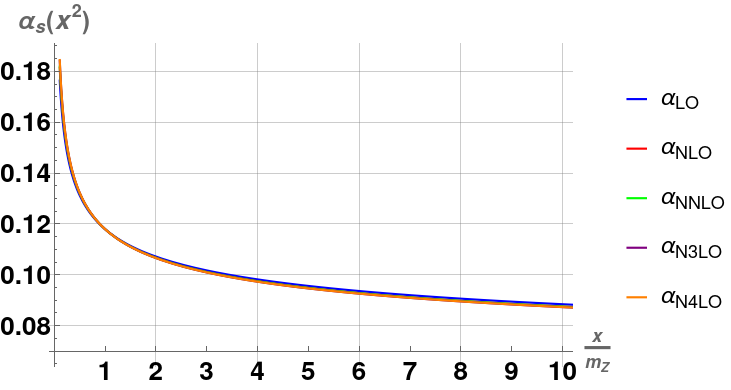
\includegraphics[width=\textwidth]{figures/alpha_running.png}
    \caption{Energy dependence of the strong coupling $\alpha_s$}
    \label{fig:alpha_running}
\end{figure}

\begin{figure}[htbp] 
    \centering
    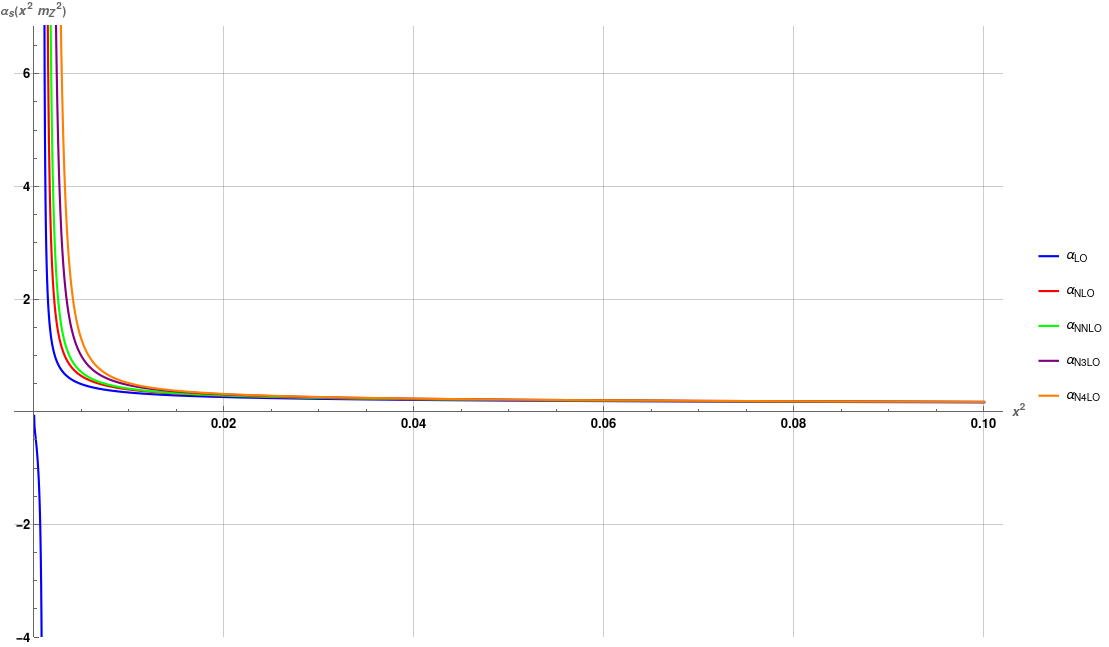
\includegraphics[width=\textwidth]{figures/alpha_zoom.png}
    \caption{Zoom-in at low energies of the strong running coupling $\alpha_s$ at different orders}
    \label{fig:alpha_zoom}
\end{figure}

In \cref{fig:alpha_zoom} wee see that at low energies the running coupling $\alpha_s$ is large and diverges at a finite 
energy (the so called Landau pole), this is a sign of the non-perturbative nature of QCD at low energies.
\end{document}